\chapter{Kiểm thử, đánh giá}

\section{Kiểm thử các thuật toán}
\subsection{Thuật toán mã hóa đối xứng}

Plaintext: \texttt{DaiHocGiaoThongVanTaiTPHCM} \\
Key: \texttt{LeHuynhAnhKhoi24}

Kiểm tra thuật toán tự triển khai từ đầu với 2 mode \texttt{ECB} và \texttt{CFB}, so sánh cách triển khai từ đầu với thư viện chuẩn, dùng vector khởi tạo cố định.

\begin{figure}[H]
	\centering
	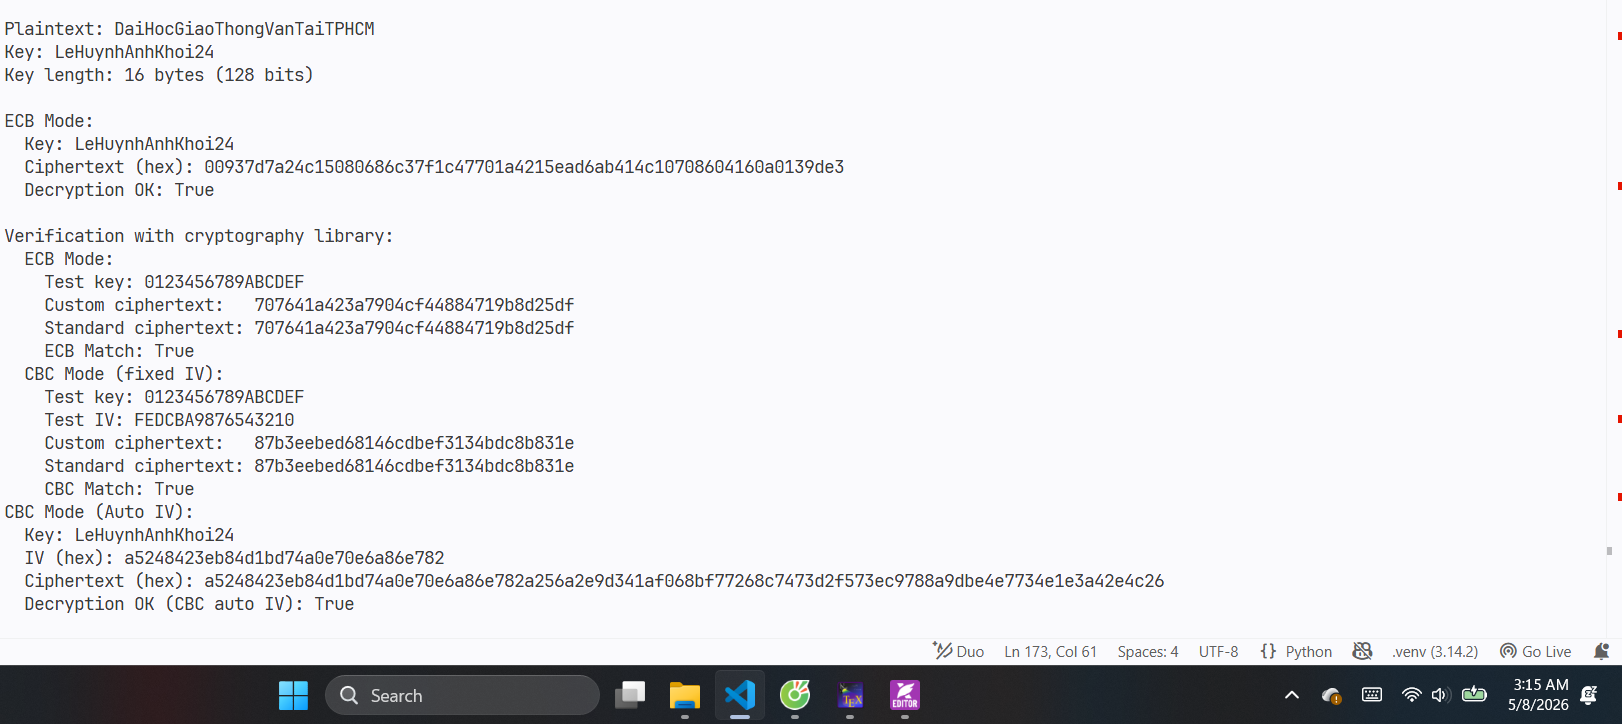
\includegraphics[width=\textwidth]{test_screenshot/aes.png} 
	\caption{Ảnh chụp màn hình kiểm thử SHA-256} 
	\label{fig:aes-test}
\end{figure}

\subsection{Thuật toán mã hóa bất đối xứng}

Alice gửi cho Bob thông điệp Message = \texttt{Toi\_la\_sinh\_vien\_nam\_2\_UTH}, được mã hóa bằng khóa công khai của Bob. Chính vì thế, đoạn thông điệp được mã hóa này chỉ được giải mã bằng khóa riêng của Bob.

\begin{figure}[H]
	\centering
	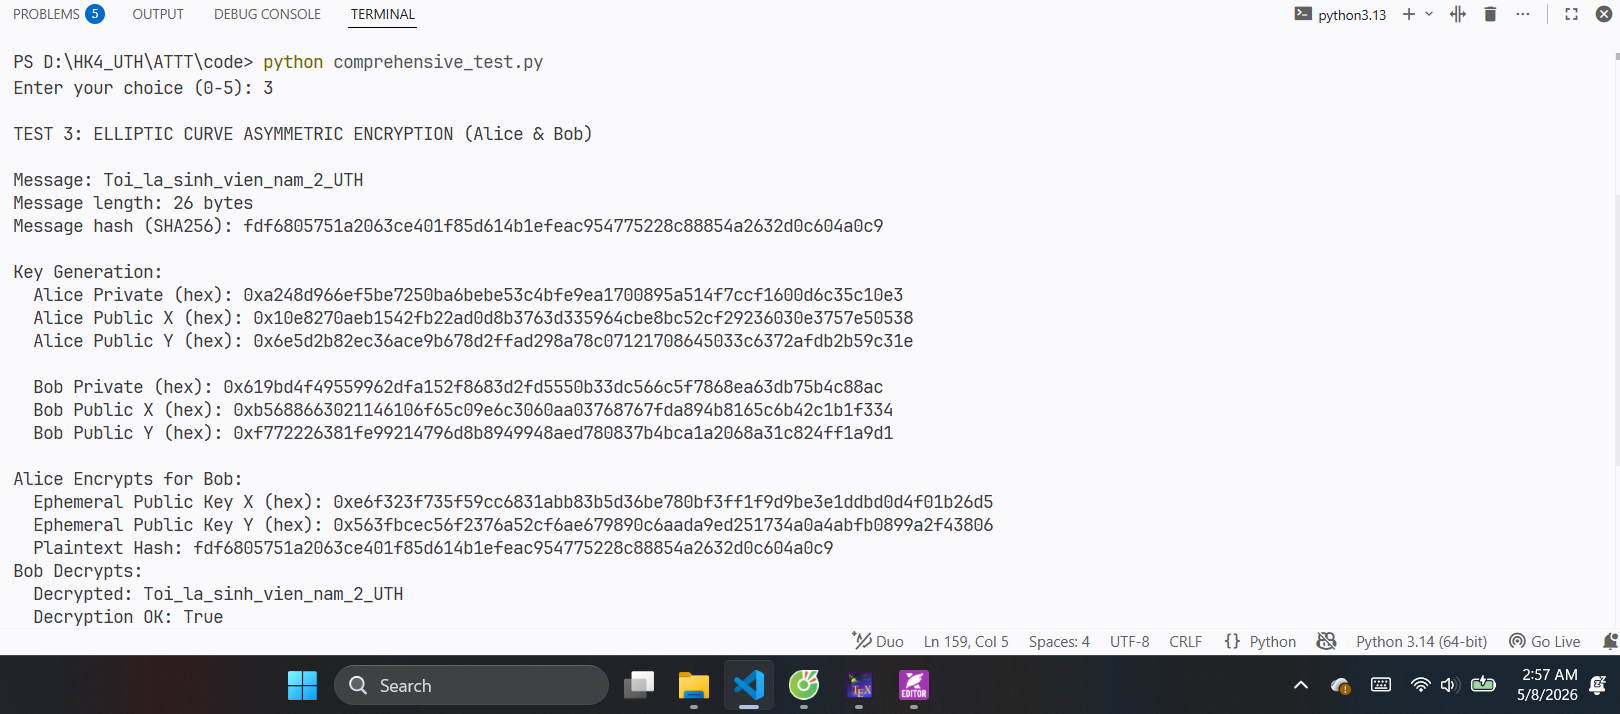
\includegraphics[width=\textwidth]{test_screenshot/asymmetric.png} 
	\caption{Ảnh chụp màn hình kiểm thử Mã hóa bất đối xứng} 
	\label{fig:ecc-test}
\end{figure}

\subsection{Hàm băm SHA-256}
Plaintext1: \texttt{LeHuynhAnhKhoiUTHDL24}.\\
Plaintext2: \texttt{LeHuynhAnhKhoiUTH\_DL24}

So sánh kết quả băm của hai Plaintext trên, và đối chiếu hàm băm tự triển khai so với hàm băm SHA-256 từ thư viện \texttt{hashlibs}:

\begin{figure}[H]
	\centering
	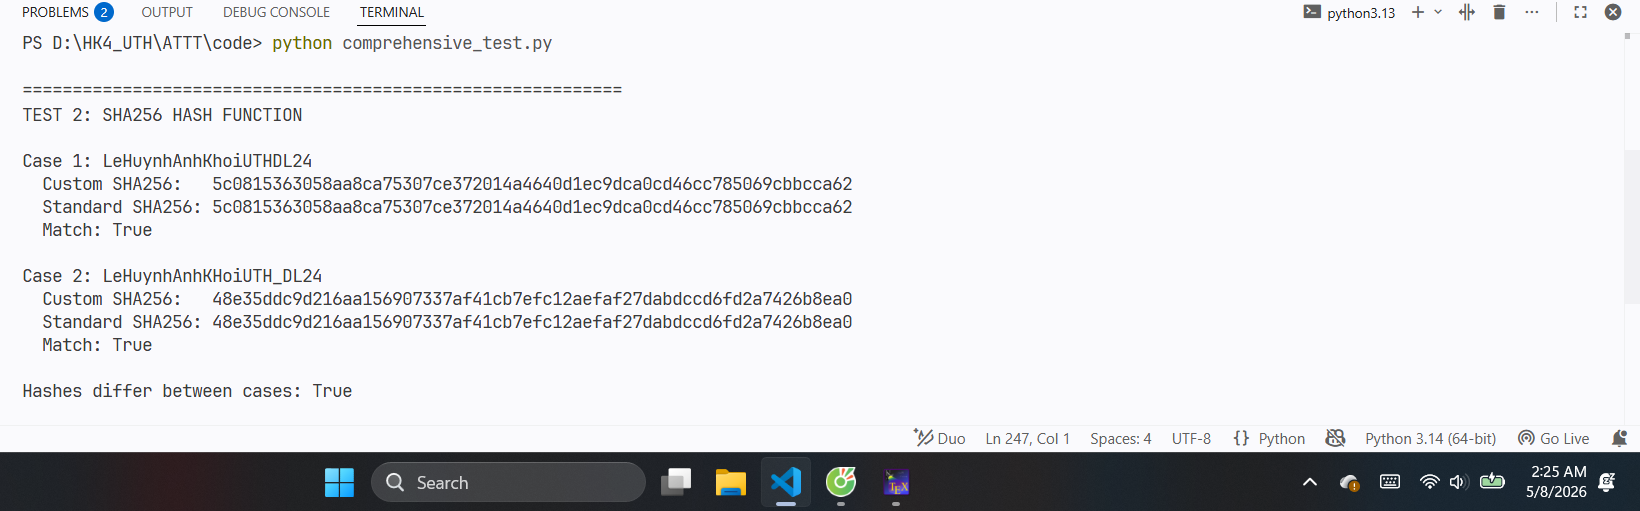
\includegraphics[width=\textwidth]{test_screenshot/sha-256.png} 
	\caption{Ảnh chụp màn hình kiểm thử SHA-256} 
	\label{fig:sha-test}
\end{figure}

\subsection{Thuật toán chữ ký số}

Alice cần gửi thông điệp \texttt{LeHuynhAnhKhoi\_UTH\_DL24} đã được ký đến Bob. Khi Bob nhận, sẽ dùng khóa chung để xác thực bản mã kèm theo chữ kí của Alice, nếu khớp nhau thì tức là Bob đã xác thực thành công tin nhắn được gửi từ Alice.

Ngoài ra, bản kiểm thử này còn đưa ra các trường hợp quá trình xác thực không hợp lệ:
\begin{enumerate}[label=\textbf{Trường hợp \arabic*.}, leftmargin = 4.5cm]
	\item Thông điệp bị thay đổi trong quá trình truyền đến Bob
	\item Sử dụng khóa công khai không đúng
	\item Bản thông điệp đính kèm chữ ký đã có sự thay đổi trong quá trình truyền đến Bob
\end{enumerate}

\begin{figure}[H]
	\centering
	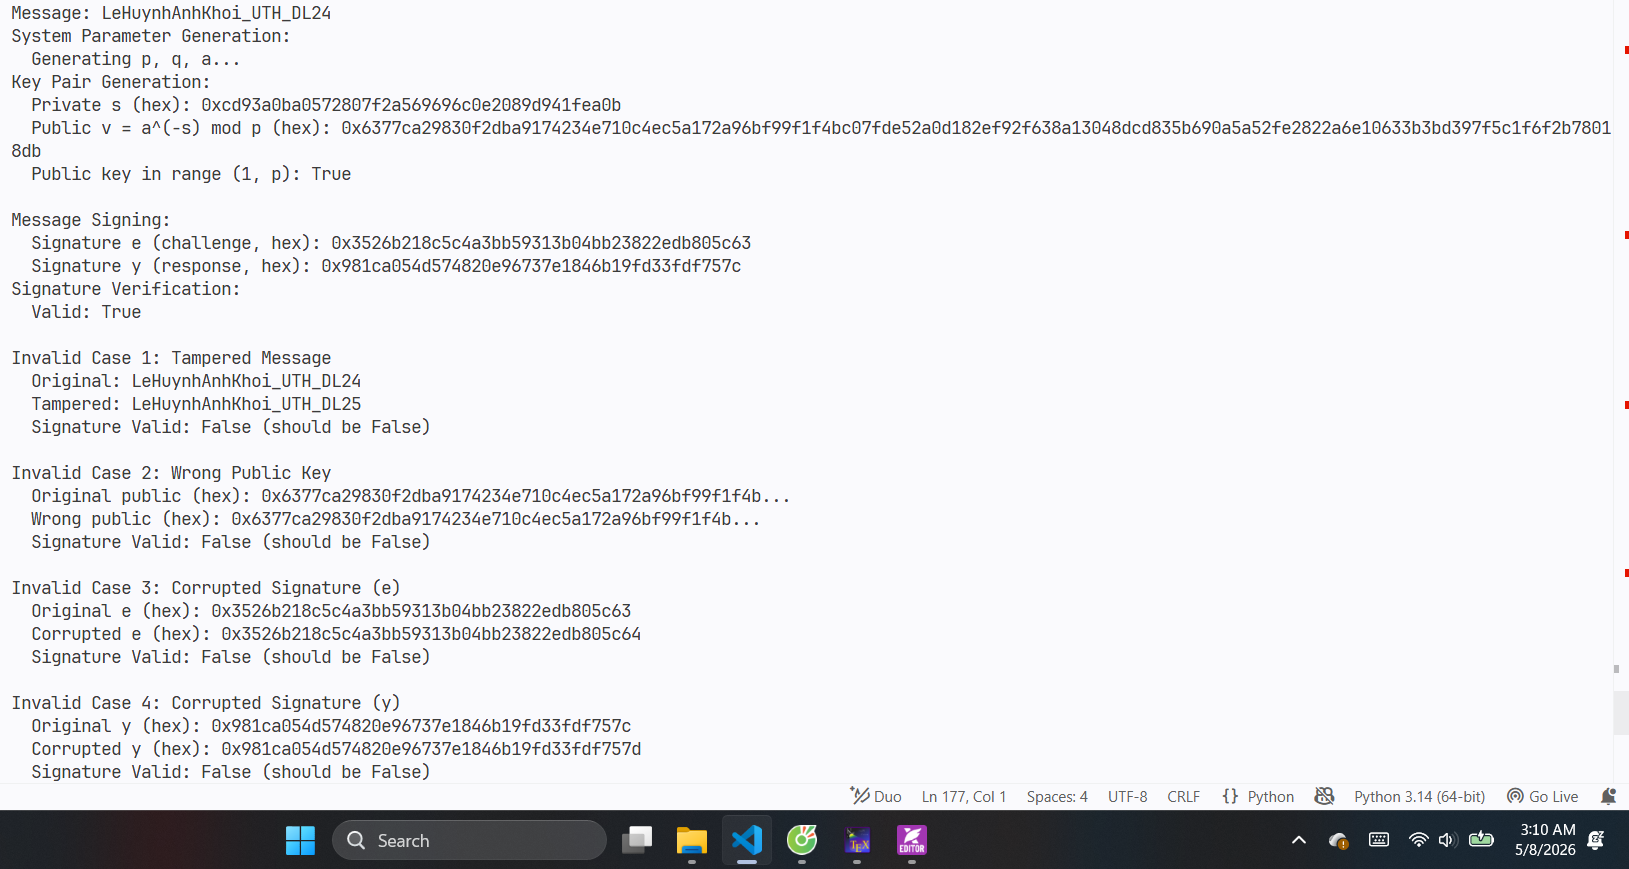
\includegraphics[width=\textwidth]{test_screenshot/schnorr.png} 
	\caption{Ảnh chụp màn hình kiểm thử Thuật toán chữ ký số} 
	\label{fig:schnorr_test}
\end{figure}
\section{Tổng hợp kết quả Demo}
\begin{table}[H]
	\centering
	\small
	\caption{Bảng tổng hợp kịch bản kiểm thử các thuật toán mật mã}
	\label{tab:kich-ban-test}
	\begin{tabularx}{\textwidth}{|l|X|X|c|}
		\hline
		\textbf{Thuật toán} & \textbf{Kịch bản Demo} & \textbf{Kết quả kỳ vọng} & \textbf{Kết quả thực tế} \\
		\hline
		\textbf{AES} & Kiểm tra 2 chế độ ECB và CFB & Kết quả mã hóa trùng khớp hoàn toàn giữa hàm tự triển khai và thư viện chuẩn. & \textbf{Pass} \\
		\hline
		\textbf{EC} & Alice mã hóa thông điệp bằng khóa công khai của Bob. & Chỉ có khóa riêng của Bob mới giải mã được chính xác thông điệp gốc. & \textbf{Pass} \\
		\hline
		\textbf{SHA-256} & Băm 2 chuỗi tương tự nhau (chỉ khác dấu \texttt{\_}) và so sánh với thư viện \texttt{hashlib}. & Hai kết quả băm khác biệt hoàn toàn (hiệu ứng thác đổ) và khớp với \texttt{hashlib}. & \textbf{Pass} \\
		\hline
		\textbf{Schnorr} & Ký và xác thực tin nhắn. Kiểm tra các lỗi: sửa đổi tin nhắn, sai khóa, sửa đổi chữ ký. & Xác thực thành công khi dữ liệu đúng; báo lỗi chính xác trong 3 trường hợp sai phạm. & \textbf{Pass} \\
		\hline
	\end{tabularx}
\end{table}

\section{Bảng đánh giá hiệu năng}

Mỗi thuật toán sẽ được đánh giá thông qua thực hiện các tác vụ chính, với kích thước tăng dần đều. Sử dụng thư viện \texttt{timeit} để đánh giá.

\begin{table}[H]
	\centering
	\small % Giúp bảng dễ thở hơn trong không gian hẹp
	\setlength{\tabcolsep}{4pt} % Thu hẹp khoảng cách giữa các cột một chút
	\caption{Đánh giá hiệu năng cho mỗi thuật toán}
\begin{tabularx}{\textwidth}{|l|l|X|r|r|r|}
		\hline
		Thuật toán & Tác vụ & Kích thước dữ liệu & Min (ms) & Max (ms) & Avg (ms) \\
		\hline
		AES & Mã hóa + Giải mã CBC & Bản rõ ASCII 64 byte & 5.8649 & 8.1550 & 6.6234 \\
		AES & Mã hóa + Giải mã CBC & Bản rõ ASCII 256 byte & 20.3539 & 22.5208 & 21.1727 \\
		AES & Mã hóa + Giải mã CBC & Bản rõ ASCII 1024 byte & 79.1453 & 88.3546 & 83.6214 \\
		AES & Mã hóa + Giải mã CBC & Bản rõ ASCII 4096 byte & 319.9004 & 367.3764 & 340.5001\\ \hline
		SHA256 & Băm tin nhắn & Tin nhắn bytes 64 byte & 0.5515 & 0.7125 & 0.6482 \\
		SHA256 & Băm tin nhắn & Tin nhắn bytes 256 byte & 1.2929 & 1.6227 & 1.5061 \\
		SHA256 & Băm tin nhắn & Tin nhắn bytes 1024 byte & 4.5049 & 5.3752 & 4.9595 \\
		SHA256 & Băm tin nhắn & Tin nhắn bytes 4096 byte & 12.1024 & 18.4987 & 14.5991 \\
		\hline
		EC\_Asymmetric & Mã hóa + Giải mã & Tin nhắn ASCII 8 byte & 17.6138 & 22.6687 & 19.6769 \\
		EC\_Asymmetric & Mã hóa + Giải mã & Tin nhắn ASCII 16 byte & 20.4318 & 27.6520 & 23.6515 \\
		EC\_Asymmetric & Mã hóa + Giải mã & Tin nhắn ASCII 32 byte & 27.3686 & 32.7380 & 29.6489 \\
		EC\_Asymmetric & Mã hóa + Giải mã & Tin nhắn ASCII 64 byte & 35.3422 & 45.1091 & 41.5510 \\
		\hline
		Schnorr & Ký số + Xác minh & Tin nhắn ASCII 32 byte & 1.2534 & 1.7206 & 1.4142 \\
		Schnorr & Ký số + Xác minh & Tin nhắn ASCII 256 byte & 2.8381 & 3.2243 & 2.9988 \\
		Schnorr & Ký số + Xác minh & Tin nhắn ASCII 1024 byte & 7.0937 & 8.4677 & 7.8106 \\
		Schnorr & Ký số + Xác minh & Tin nhắn ASCII 4096 byte & 25.5379 & 28.0817 & 26.7372 \\
		\hline
	\end{tabularx}
	\label{tab:danh-gia-hieu-nang-4-muc-do}
\end{table}

\section{So sánh các thuật toán}

\begin{table}[H]
	\centering
	\small
	\setlength{\tabcolsep}{3pt} % Ép khoảng cách giữa các cột nhỏ lại tối đa
	\begin{tabularx}{\textwidth}{|l|c|X|X|X|c|X|} % Chuyển 4 cột nội dung thành X để ép xuống hàng
		\hline
		\textbf{Thuật toán} & \textbf{Phân loại} & \textbf{Ứng dụng} & \textbf{Kích thước khóa} & \textbf{Kích thước Output} & \textbf{Giải mã} & \textbf{Tốc độ (Avg)} \\
		\hline
		\textbf{AES} & Đối xứng & Mã hóa dữ liệu lưu trữ, bảo mật kênh truyền. & 128/192/ 256 bit & Bằng Input + Padding & Có & Trung bình (6.6ms/64B $\rightarrow$ 340.5ms/
		4KB) \\
		\hline
		\textbf{SHA-256} & Hàm băm & Kiểm tra toàn vẹn, lưu trữ mật khẩu. & Không dùng khóa & Cố định 256 bit (32 byte) & Không & Rất nhanh (0.6ms/64B $\rightarrow$ 14.6ms/4KB
		) \\
		\hline
		\textbf{EC\_Asym} & Bất đối xứng & Trao đổi khóa, mã hóa thông điệp ngắn. & Thường 256 bit & Phụ thuộc đường cong (lớn hơn Input) & Có & Rất chậm (41.5ms chỉ cho 64 byte) \\
		\hline
		\textbf{Schnorr} & Chữ ký số & Xác thực danh tính, chống chối bỏ. & Cặp khóa ECC & Cố định (thường 64 byte cho r, s) & Không & Nhanh (1.4ms/32B $\rightarrow$ 26.7ms/4KB) \\
		\hline
	\end{tabularx}
	\caption{So sánh tổng quan 4 phương pháp mật mã đã triển khai.}
	\label{tab:so-sanh-tong-quan}
\end{table}

\section{Nhận xét và Đánh giá tổng quan}

Kết quả thực nghiệm cho thấy mỗi thuật toán đều mang một đặc tính hiệu năng riêng biệt:

\begin{itemize}
	\item \textbf{Nhanh và ổn định nhất (SHA-256 \& Schnorr):} SHA-256 cho tốc độ băm cực nhanh bất chấp kích thước đầu vào. Tương tự, lược đồ chữ ký số Schnorr nhanh hơn nhiều so với lược đồ DSA, RSA nhờ vào tính đơn giản.
	\item \textbf{Cân bằng và tối ưu cho dữ liệu lớn (AES):} Tốc độ ở mức trung bình nhưng cực kỳ ổn định khi quy mô dữ liệu tăng lên.
	\item \textbf{Chậm nhất nhưng an toàn (Mã hóa bất đối xứng sử dụng đường cong Elliptic):} Việc mã hóa/giải mã bằng đường cong Elliptic tốn rất nhiều thời gian và tài nguyên, nhưng chúng lại là phương thức an toàn nhất để giải quyết bài toán trao đổi khóa ban đầu.
\end{itemize}

Trong các hệ thống doanh nghiệp thực tế, các hệ thống bảo mật luôn áp dụng phương pháp sử dụng kết hợp giữa các hệ mật mã khác nhau:
\begin{itemize}
	\item Chấp nhận tốc độ chậm của ECC để trao đổi một "Khóa phiên" (Session Key) an toàn.
	\item Sự ổn định của AES cùng Khóa phiên để mã hóa toàn bộ thông điệp, dữ liệu lớn.
	\item Tận dụng tốc độ nhanh của SHA-256 và Schnorr để ký - xác thực, đảm bảo tính toàn vẹn cũng như tính không thoái thác.
\end{itemize}
